\documentclass[11pt]{article}

%%%%%%%%%%%%%%Include Packages%%%%%%%%%%%%%%%%%%%%%%%%%%
\usepackage{xcolor}
\usepackage{mathtools}
\usepackage[a4paper, total={6in, 8in}, margin=1.25in]{geometry}
\usepackage{amsmath}
\usepackage{amssymb}
\usepackage{paralist}
\usepackage{rsfso}
\usepackage{amsthm}
\usepackage{wasysym}
\usepackage[inline]{enumitem}   
\usepackage{hyperref}
\usepackage{tocloft}
\usepackage{titlesec}
\usepackage{colortbl}
\usepackage{wrapfig}
\usepackage{pdfpages}
%%%%%%%%%%%%%%%%%%%%%%%%%%%%%%%%%%%%%%%%%%%%%%%%%%%%%%%%



\begin{document}
%\begin{wrapfigure}[9]{r}{0.3\textwidth}
%  \begin{center}
%  \vspace{-15pt}
%    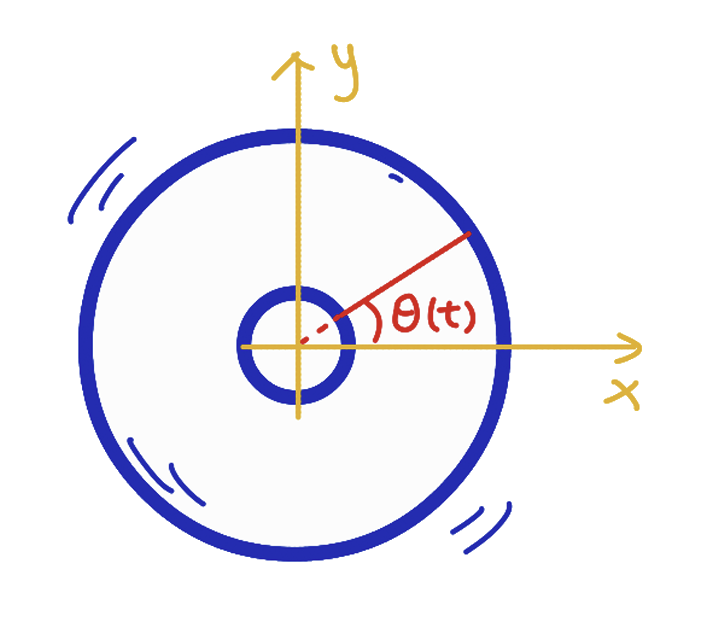
\includegraphics[scale=0.19]{disk}
%  \end{center}
%\end{wrapfigure}
\Large \noindent \textbf{Physics 1A Review Session}\\
\normalsize
Department of Physics and Astronomy, UCLA\\
\noindent\rule{8cm}{0.4pt}\\
\textbf{Problem 1}: Jinyan throws a marker into the air, with initial speed $v_0=2$ m/s at an angle $\phi=60^\circ$ with respect to the ground as shown. It is moving through the air as well as spinning (about an axis through its center of mass right at the middle of the marker). 
\begin{center}
\includegraphics[scale=0.69]{p1}
\end{center}
The marker lands 2 meters (in horizontal distance) away from where it is thrown, with a final angular velocity $\omega=1$ rad/s. Find the initial height $y_0$ of the marker, the angular displacement $\theta$ of the marker over its entire journey, and the final velocity of the marker. Neglect all forms of friction.\\



\newpage
\noindent\textbf{Problem 2}: Jinyan throws a $0.1\,$kg stress ball against a metal rod. 
\begin{center}
\includegraphics[scale=0.69]{p2}
\end{center}
The stress ball travels with a speed $10$ m/s in the positive-$x$ direction and hits the metal rod at a distance $L=1$ meter from which the rod is hinged. You can neglect the gravitational force acting on the ball (so the ball travels to the right in a straight line with constant speed). \footnote{Even though there are many sub-problems in this problem, most of them are one-line calculation. Make sure you have the correct units written down for your final answers.}\\


\noindent \textbf{(a)} The rod (approximated as an $1$-dimensional object) has a non-uniform line-density $\lambda = 10y$ (with unit kilogram per meter), so the upper end of the rod is heavier. Find the total mass, center of mass, and moment of inertia of the rod (rotating around the top hinge).\\

\noindent\textbf{(b)} At the moment the ball hits the rod, it drops to the ground vertically, but the rod rotates counterclockwise with an angular velocity $\omega$. Find $\omega$.\\

\noindent\textbf{(c)} The rod rotates subject to gravity. Find the maximal height that the center of mass of the rod can reach. \\


\noindent\textbf{(d)} [A little challenging and requires a little bit of high-school geometry] Find the torque acting on the rod by gravity when the center of mass gets to its maximal height. 



\newpage
\noindent\textbf{Problem 3}: Two stars are separated by a distance $2d$ deep in space. Jinyan as an astronaut is floating in space with some initial velocity $v_0$ towards the positive-$x$ direction as shown. \\
\begin{center}
\includegraphics[scale=0.69]{p3}
\end{center}
\noindent \textbf{(a)} The two stars have the same mass $M$, and Jinyan has mass $m$. Let us hypothetically assume that the two stars are fixed at their current position, not moving, while Jinyan is trapped by the gravity of the two stars. Also assume that Jinyan carries no thruster on him (so the only acceleration that he experiences is due to gravity). Find the minimal initial speed $v_0$ needed such that he can escape from the stars (going from the current position at $x = x_0$ to $x \to \infty$).\footnote{Use energy conservation and use the gravitational force that you learned in Chapter 13. Treat this problem as a one-dimensional problem, that Jinyan is only allowed to move along the $x$-axis.} \footnote{I realized that I might have made this problem too difficult when I was writing the solution to it. You will need to use some symmetry argument to find that the net force (by the two stars) acting on Jinyan is 
\begin{align*}
\vec{F}_{\text{net}} = -\frac{2GMm}{x^2+d^2}\frac{x}{\sqrt{x^2 + d^2}} \hat{x}\,.
\end{align*}
Then you can start from here, the net force, and use conservation of energy to find the minimal speed needed for me to escape. The rest of the problem shouldn't be too difficult, other than some technicalities needed in computing integrals, I think. 
} \footnote{
You will need this:
\begin{align*}
\frac{d}{dx}\left(\frac{1}{\sqrt{x^2 + d^2}}\right) = -\frac{x}{(x^2 + d^2)^{3/2}}\,.
\end{align*}
}\\

\noindent\textbf{(b)} Hypothetically, if Jinyan were unable to escape,\footnote{So in that case you won't be able to see him again in the Physics department, sad ...} he would travel through the origin in the coordinate system at some later time. Explain qualitatively why that would happen. Show quantitatively that the origin is a stable equilibrium position. \\

\noindent\textbf{(c)} Approximate the gravitational potential energy that Jinyan would feel around the origin (stable equilibrium). That is, compute the first few terms in Taylor expansion of $U(x)$ around $x =0$, given that $\Delta x$ is small. How does this compared to the standard spring potential energy?

\newpage
\noindent\textbf{Problem 4}: Jinyan is playing with two electrons.\footnote{Unfortunately, I am not an experimentalist.} \footnote{This problem is a baby version of electron-electron scattering. In quantum field theory, electron scattering (Moller scattering) can be described by computing the second-order scattering-matrix element of the Feynman diagram depicted in the cartoon,
\begin{align*}
S^{(2)} = &\frac{ie^2 g_{\mu\nu}}{(2\pi)^4} \int d^4x \,d^4y\,  d^4k\,\frac{e^{-ik(x-y)}}{k^2 + i\epsilon}\,
\frac{\bar{u}_{r_3,\alpha}(\vec{p}_3)\, e^{ip_3y}\, \gamma^\mu_{\alpha\beta}\, \bar{u}_{r_4,\delta}(\vec{p}_4) \, e^{ip_4x} \,\bar{u}_{r_1,\alpha}(\vec{p}_1)\, e^{ip_1y}\, \bar{u}_{r_2,\delta}(\vec{p}_2) \, e^{ip_2x}\, \gamma^\nu_{\delta\epsilon}}{m^{-2}V^2\sqrt{E_{\vec{p}_3}E_{\vec{p}_3}E_{\vec{p}_1}E_{\vec{p}_2}}}
\,,
\end{align*}
with $\vec{p}_i$ denoting the momentum of the electrons. After the integration, $S^{(2)}$ has a factor regarding the conservation of total momentum,
\begin{align*}
\int d^4x\, e^{-ix(p_1-p_3)} e^{ip_4x} e^{ip_2x} = (2\pi)^4 \, \delta^{(4)}(p_3+p_4 - p_1 - p_2)\,.
\end{align*} 
Physicists have spent billions of money in studying collision of particles. 
}\\
\begin{center}
\includegraphics[scale=0.69]{p4}
\end{center}
Electron-electron scattering is considered as an elastic ``collision." The two incoming electrons, each with mass $m$, have initial velocity $\vec{v}_a = (v_{a,x}, v_{a,y})$ and $\vec{v}_b = (v_{b,x}, v_{b,y})$. Jinyan put a detector at the position shown in the figure, at an angle $\theta_1$. The detector beeps and is able to capture one of the two outgoing electrons. He needs your help to find the angle $\theta_2$ to put the second detector to capture the other electron. Find $\theta_2$ if we have 
\begin{align*}
\vec{v}_a = \left(1+\frac{\sqrt{3}}{2}\,,\ \frac{\sqrt{3}}{2}\right)\,\,\text{m/s} \,,\qquad
\vec{v}_b = \left(1-\frac{\sqrt{3}}{2}\,,\ \frac{\sqrt{3}}{2}\right)\,\text{m/s} \,,\qquad \theta_1 = 0^\circ\,.
\end{align*}



\newpage
English is not my first language, so if you find any ungrammatical thing in this solution that makes you confused, let me know and I can clarify it ...\\

\noindent\textbf{Problem 1}: This is a very standard kinematics problem. The way to solve this problem is by decomposing the spatial motion into $x$- and $y$-components. The spinning of the marker is a separate thing that will be dealt with later, and it does not affect at all the translational motion of the marker. \\

The only force that the marker experiences is the gravitational force, acting right at the center of mass of the marker (right at the middle of the marker). Therefore, we have 
\begin{align*}
\vec{a} = (0,\, -9.8)\,\text{m/s}^2\,.
\end{align*}
This is a constant acceleration, from which we know that we should apply kinematic equations, rather than doing fancy energy conservation or momentum conservation. You can do the problem using energy conservation, but not recommended. For initial velocity 
\begin{align*}
\vec{v}_0 = (2\cos(60^\circ),\, 2\sin(60^\circ))\,\text{m/s} =(1,\, \sqrt{3})\,\text{m/s} \,. 
\end{align*}
Let me define the origin to the point there I throw the marker, so $(x_0,y_0 )= (0,0)$ m. Now we write down the $x$- and $y$-direction kinematic equations and plug in the numbers, 
\begin{align*}
x = \frac{1}{2}a_x t^2 + v_{0,x}t  + x_0 =0 + t + 0 =t\,,\\
y = \frac{1}{2}a_y t^2 + v_{0,y}t  + y_0 = -4.9t^2 + \sqrt{3}t+ 0  = -4.9 t^2 + \sqrt{3} t\,.
\end{align*}
We see that, when $t = 2$ seconds, we get $x = 2$ meters. Therefore the time label that the marker reaches the ground is $t = 2$ seconds. Then, 
\begin{align*}
y(t=2) = -4.9 \cdot 2^2 + \sqrt{3} \cdot 2 = - 16.14\,.
\end{align*}
From here we deduce that the total vertical displacement that the marker has traveled is $16.14$ meters downwards, the marker is thrown at an initial height $16.14$ above the ground. \\

Now what about the total angular displacement $\theta$? Again, the only force acting on the marker is the gravitational force, which acts exactly at the center of mass of the marker, and is also where the rotation\ axis of the marker is located at. The ``lever arm" for calculating the torque due to gravitational force is thus zero, so $\tau_{\text{net}} = \tau_g = 0 \cdot F_g = 0$. We conclude that the angular acceleration of the marker is zero, so 
\begin{align*}
\theta = \frac{1}{2}\alpha t^2 + \omega_0 t + \theta_0 = \omega_0 t  + \theta_0\,.
\end{align*}
Here we have $\omega_0 = 1$ rad/s given in the problem, at $t = 2$ seconds, the angular displacement is 
\begin{align*}
\theta - \theta_0 = 2 \,\text{rad}\,.
\end{align*}

Final velocity at the moment it lands is calculated via
\begin{align*}
v_{x,f} = v_{x,0} + a_x t = v_{x,0} = 1 \,\text{m/s} \,,\qquad
v_{y,f} = v_{y,0} + a_y t = \sqrt{3}-9.81\cdot 2 = -17.89\,\text{m/s}\,.
\end{align*}
Therefore, $|\vec{v}_f| = \sqrt{1^2 + (17.88)^2} = 17.91$\,m/s. 
No calculus needed.\\

\newpage
\noindent\textbf{Problem 2}: The total mass of the rod is 
\begin{align*}
M = \int dm = \int_{0}^1 \lambda\, dy = \int_0^1 10y \, dy =5 \,\text{kg}\,.
\end{align*}
The center of mass is 
\begin{align*}
\vec{r}_{\text{com}} = \left(0\,\text{m}\,,\ y_{\text{com}}\right)\,.
\end{align*}
Here we calculate
\begin{align*}
y_{\text{com}} =\frac{1}{m} \int y \, dm =\frac{1}{m} \int_0^1 y \lambda \,dy =\frac{10}{5} \int_0^1 y^2 \, dy = \frac{2}{3} \,\text{m}\,.
\end{align*}
Lastly, we calculate the moment of inertia, 
\begin{align*}
I = \int |r_\perp|^2\, dm = \int_0^1 (1-y)^2 \, \lambda \, dy =  \int_0^1 (1-y)^210y \, dy =10 \int_0^1 y-2y^2 + y^3\, dy = \frac{5}{6} \, \text{kg\,m}^2\,.
\end{align*}
The ball hits the rod, which is a ``collision" event so we use conservation of angular momentum. Before the collision, only the ball is moving, so $L_{i} = rp \sin(\theta)$ where $\theta$ is the angle between the lever arm $\vec{r}$ and the momentum vector $\vec{p}$ of the ball. The ball is traveling horizontally in space, so $\vec{p} = m v \hat{x}$, whereas the lever arm is vertical (aligned with the metal rod), thus the angle between them is $90^\circ$. After the collision, the ball contributes zero angular momentum (because it just falls to the ground, linear momentum is downward, lever arm is also downward, so angle between the two is zero), but the rod is rotating, contributing $L_f = I\omega$, thus we write
\begin{align*}
rp\sin(\theta)=rmv &= I\omega\,,
\end{align*}
then plug in $r = 1$\,m, $m = 0.1$\,kg, $v = 10\,$m/s, and $I = 5/6$\,kg\,m, we obtain 
\begin{align*}
\omega = \frac{6}{5} \,\text{rad}/s\,.
\end{align*}
The next one is about rotation of the rod. We should use energy conservation to solve the problem, this is because the torque due to gravitational force is not constant, 
\begin{align*}
\tau_g = \vec{r}\times \vec{F}_g = r F_g \sin(\theta)\,,
\end{align*}
with $\theta$ (the angle between the vertically downwards gravitational force and the rod, which is physically rotating) changing, so $\tau_g$ being non-constant prevents us from applying kinematic equations to solve the problem. Using conservation of energy, 
\begin{align*}
K_\text{rot,i} + U_{g,i} &=
K_\text{rot,f} + U_{g,f}\,,\\
\frac{1}{2}I\omega_i^2 + Mg h_i&=\frac{1}{2}I\omega_f^2 +Mg h_f\,, 
\end{align*}
where $h_i =2/3$\,m is the initial height where we can find the center of mass of the rod, and $h_f$ is the final height where we can find the center of mass. Also, $\omega_i = 12$ rad/s as we just computed, and $\omega_f = 0$ when the center of mass gets to its maximal height. I am lazy, I take $g = 10$ m/s$^2$. 
\begin{align*}
\frac{1}{2}\cdot\frac{1}{12}\cdot \left(
\frac{6}{5}
\right)^2 + \frac{1}{2}\cdot 10 \cdot \frac{2}{3} = \frac{1}{2}\cdot 10 \cdot h_f\,,
\end{align*}
from which we get $h_f = 0.679$ meters. This is a $0.013$ meters displacement from the initial height of the center of mass. \\

The very last part requires us to find the angle $\theta$ between the rod and the vertical when the center of mass gets to its maximal height. We use the geometry to find the angle between the direction of lever arm $\vec{r}$ and the direction of gravitational acceleration $\vec{g}= -g \hat{y}$,  
\begin{align*}
\theta = \arccos\left(\frac{1-0.679 }{1-2/3}\right) = 15.6^\circ\,.
\end{align*}
Now we can compute
\begin{align*}
\tau_g = rF_g\sin(\theta) = 1 \cdot \frac{1}{2} \cdot 10 \cdot \sin(15.6^\circ)\,\,\text{Nm} = 1.35\,\text{Nm}\,.
\end{align*}
I am being lazy again and take $g = 10$ m/s$^2$.

\newpage
\noindent\textbf{Problem 3}: Using the coordinate system as shown in the figure, the star at $y = d$ exerts a gravitational force
\begin{align*}
\vec{F}_t = -\frac{GM m}{(x^2+d^2)^{3/2}} \left( x\hat{x}-d\hat{y}\right)\,,
\end{align*}
and the star at $y = -d$ exerts a gravitational force
\begin{align*}
\vec{F}_b = -\frac{GM m}{(x^2+d^2)^{3/2}} \left( x\hat{x}+d\hat{y}\right)\,.
\end{align*}
Thus the net force acting on Jinyan is 
\begin{align*}
\vec{F}_{\text{net}} = \vec{F}_t + \vec{F}_b = -\frac{2GM mx}{(x^2+d^2)^{3/2}} \hat{x}\,.
\end{align*}
From here we can find the gravitational potential energy that Jinyan experiences, via $\vec{F}_{\text{net}} = -dU/dx\ \hat{x}$, so we write 
\begin{align*}
U(x) = \int \frac{2GMmx}{(x^2 + d^2)^{3/2}}\, dx\,.
\end{align*}
This seems to be a very difficult integral, but notice that 
\begin{align*}
\frac{d}{dx}\left(\frac{1}{\sqrt{x^2 + d^2}}\right) = -\frac{x}{(x^2 + d^2)^{3/2}}\,.
\end{align*}
We find 
\begin{align*}
U(x) = -\frac{2GMm}{\sqrt{x^2 + d^2}} +\text{constant}\,.
\end{align*}
As we have discussed, the constant in energy does not matter, we can always wipe it out by redefinition. thus 
\begin{align*}
U(x) = -\frac{2GMm}{\sqrt{x^2 + d^2}}\,.
\end{align*}
To escape to infinity, I want to have enough initial kinetic energy 
\begin{align*}
K = \frac{1}{2}mv_0^2
\end{align*}
such that
\begin{align*}
K \geq U(x= \infty) - U(x=x_0)
\end{align*}
We see that
\begin{align*}
\lim_{x\to \infty} U(x) = 0\,,
\end{align*}
Thus the minimal amount of $K$ corresponds to 
\begin{align*}
K_{\min} = \frac{2GMm}{\sqrt{x_0^2 + d^2}}\,.
\end{align*}
and thus the minimal speed needed is
\begin{align*}
v_0 = \left(\frac{4GM}{\sqrt{x_0^2 + d^2}}\right)^{1/2}\,,
\end{align*}
which is surprisingly independent on $m$, the mass of Jinyan, even though he is not that heavy. \\

Now if I were unable to escape, since I am trapped by the gravity, I will be initially moving to the right (positive-$x$ direction), the gravitational forces by the two stars will slow me down, and gradually pull me back to the left, passing through the origin, going to the left. Then after a while, when I get too far to the left, the gravitational forces will pull me to the right, and so I will get back to the origin, continue going to the right. I will end up oscillating around the origin due to the gravitational forces, and that is why the origin is a stable equilibrium position (that is, any small perturbation from this equilibrium position will end up going back to the equilibrium position).\\

To show that the origin is an equilibrium position, 
\begin{align*}
\frac{dU}{dx}|_{x = 0} = -F_x|_{x=0} = 0\,.
\end{align*}
This we because we know that the $x$-component of the net force acting on Jinyan is
\begin{align*}
F_x = -\frac{2GMmx}{(x^2 + d^2)^{3/2}}
\end{align*}
which vanishes when $x = 0$. Now to show that this is a stable equilibrium, 
\begin{align*}
\frac{d^2 U}{dx^2}|_{x=0} = \frac{2GMm(x^2+d^2)^{3/2} - 3GMmx(x^2+d^2)^{1/2}}{(x^2+d^2)^3}|_{x = 0} = \frac{2GMm}{d^3}
\end{align*}
which is strictly positive as all variables are positive. Therefore, we conclude, quantitatively, that the origin is a static equilibrium. \\

To find the Taylor expansion of $U(x)$ around the equilibrium, we have done most of the computations, we just need to assemble them. 
\begin{align*}
U(x) &= U_0 + \frac{dU}{dx}|_{x=0}\, x + \frac{1}{2}\frac{d^2U}{dx^2}|_{x=0}\, x^2 + \text{(higher order terms)}\\
&\approx -\frac{2GMm}{d} + 0\cdot x + \frac{1}{2}\frac{2GMm}{d^3}x^2\\
&=-\frac{2GMm}{d}  + \frac{1}{2}\frac{2GMm}{d^3}x^2\,.
\end{align*}
Notice that the first term is a constant term that we can drop by redefining $U(x)$, again because a constant term in energy has no physical meaning. Then we will be left with
\begin{align*}
U(x) = \frac{1}{2}\frac{2GMm}{d^3} x^2\,,
\end{align*}
with $x = x-0 = \Delta x$, and thus this is equivalent to having a spring with spring constant $k = 2GMm/d^3$ attached to Jinyan. This is why you would expect to see Jinyan oscillating around the origin if he was unable to escape.

\newpage

\noindent\textbf{Problem 4}: Phew$\sim$ we get to the last one, and this one seems easy. This is a collision of two objects, so my intuition tells me that I want to solve it using momentum conservation. If you have been attending my discussion sections, excellent! You should also have noticed that conservation of momentum should do the trick. \underline{In particular}, this is an elastic collision, so we want to use momentum conservation combined with energy conservation, and I expect to solve for three unknowns using three equations. Two equations from momentum conservation in the $x$- and $y$-directions, respectively, and one equation from energy conservation.\\

Here they are: The first one comes from $x$-direction momentum conservation
\begin{align*}
mv_{a,x} + mv_{b,x} = mv_1\cos(\theta_1)+ mv_2\cos(\theta_2)\,,
\end{align*}
where $v_1$ is the unknown final speed for one of the two outgoing electrons (the one detected by detector one put that $\theta_1$), and $v_2$ is the unknown final speed for the other outgoing electron, to be detected by the detector placed at the unknown angle $\theta_2$. Now in the $y$-direction, 
\begin{align*}
mv_{a,y} + mv_{b,y} = mv_1\sin(\theta_1)+ mv_2\sin(\theta_2)\,.
\end{align*}
The third one is energy conservation, 
\begin{align*}
\frac{1}{2}m(v_{a,x}^2 + v_{a,y}^2)+
\frac{1}{2}m(v_{b,x}^2 + v_{b,y}^2) =  
\frac{1}{2}mv_1^2+
\frac{1}{2}mv_2^2\,.
\end{align*}
We divide the momentum equations by $m$, and the energy equation by $m/2$, 
\begin{align*}
\begin{cases}
v_{a,x} + v_{b,x} = v_1\cos(\theta_1)+ v_2\cos(\theta_2)\\
v_{a,y} + v_{b,y} = v_1\sin(\theta_1)+ v_2\sin(\theta_2)\\
v_{a,x}^2 + v_{a,y}^2+
v_{b,x}^2 + v_{b,y}^2 =  
v_1^2+
v_2^2
\end{cases}\,.
\end{align*} 
A nice system of three equations with three unknowns, $v_1$, $v_2$, and $\theta_2$, to be solved. Let us plug in the numbers, 
\begin{align*}
\begin{cases} 
2 = v_1 + v_2\cos(\theta_2)\\
\sqrt{3} = v_2\sin(\theta_2) \\
5 = v_1^2 + v_2^2
\end{cases}\,.
\end{align*} 
%Let me combing the two momentum equations, 
%\begin{align*}
%\tan(\theta_2) = \frac{v_{a,y} + v_{b,y} - v_1\sin(\theta_1)}{v_{a,x}+v_{b,x} - v_1\cos(\theta_1)}\,.
%\end{align*}
Using the first two equations,  
\begin{align*}
(2-v_1)^2 = v_2^2 \cos^2(\theta_2)\,,\qquad
v_2^2\sin^2(\theta_2) = 3 \,.
\end{align*}
Euler said $\cos^2(\theta) + \sin^2(\theta ) = 1$, so we get
\begin{align*}
v_2^2 = 3 + (2-v_1)^2\,.
\end{align*}
Then we can use the third equation in the system to write
\begin{align*}
5-v_1^2 =v_2^2 =3+(2-v_1)^2\,,
\end{align*}
which gives $v_1 = 1$ m/s, and thus $v_2 =2$ m/s from the third equation in the system. Then finally, using the second equation of the system, 
\begin{align*}
\sqrt{3} = 2\sin(\theta_2)\,,
\end{align*}
to find $\theta_2 = 60^\circ$. Done.\\

\noindent\textbf{Treat yourself to something nice if you read this sentence, maybe a boba :)}

\end{document}


